\documentclass[a4paper]{article}

%% Language and font encodings
\usepackage[english]{babel}
\usepackage[utf8]{inputenc}
\usepackage{ragged2e}

% for figures
\usepackage{graphicx}

% for hyperlinks
\usepackage[colorlinks = true,
            linkcolor = blue,
            urlcolor  = blue,
            citecolor = blue,
            anchorcolor = blue]{hyperref}

% for pseudocode
\usepackage{algorithm}
\usepackage{algpseudocode}
% for coloring
\usepackage[usenames,dvipsnames,svgnames]{xcolor}

% bibliography
\usepackage[backend=biber,citestyle=authoryear]{biblatex}
\addbibresource{FDTD_paper.bib}

% paragraph spacing
\setlength{\parindent}{0em}
\setlength{\parskip}{0.5em}

\begin{document}

\title{Simulating electromagnetic wave propagation in ice with finite difference time domain}
\author{Ben Hills}
\maketitle

\justify
\textbf{Abstract:} Radar and seismic methods are used as geophysical techniques in many disciplines within the earth sciences. These techniques tell us something about the internal structure of a material that we can not physically see into. The utility of that knowledge is widespread. For example, geophysical methods are commonly used in the cryosphere to know the internal form of snow and ice masses, thereby giving indirect information about the accumulation and deformation of the mass

\raggedright
\section{Introduction}
Radar and seismic methods are used as geophysical techniques in many disciplines within the earth sciences. These techniques tell us something about the internal structure of a material that we can not physically see into. The utility of that knowledge is widespread. For example, geophysical methods are commonly used in the cryosphere to know the internal form of snow and ice masses, thereby giving indirect information about the accumulation and deformation of the mass
itself. 

As a project for ESS 511, Geophysical Continuum Mechanics, I will simulate these equations for electromagnetic wave propagation through ice. Starting in one dimension, I will prescribe some contrasts in the material constants that force a reflection of the wave back toward the surface. Provided that I have time I will move on to a two-dimensional model. Finally, I will discuss the practical applications of this model in glaciology research \cite{Christianson2016} as well as the general use of geophysical techniques in this field.

\section{Methods}

\subsection{Maxwell's Equations}

In this case, we can use Maxwell's curl equations to simulate the propagation of an electromagnetic wave through ice. Following , the equations are written as, 

\begin{equation}
    \nabla \times \textbf{E} = - \frac{\partial \textbf{B}}{\partial t}
    \label{eqn:E}
\end{equation}
\begin{equation}
    \nabla \times \textbf{H} = \textbf{J} + \frac{\partial \textbf{D}}{\partial t}
    \label{eqn:H}
\end{equation}

Here, \textbf{E} and \textbf{H} are the electric and magnetic fields, respectively, and t is time. All other vectors are related to \textbf{E} and \textbf{H} through the constitutive equations, 

\begin{equation}
    \textbf{B} = \mu \textbf{H} 
    \label{eqn:CM}
\end{equation}
\begin{equation}
    \textbf{D} = \epsilon \textbf{E} 
    \label{eqn:CE}
\end{equation}
\begin{equation}
    \textbf{J} = \sigma \textbf{E}   
    \label{eqn:Ohm}
\end{equation}

Equation \ref{eqn:CM} relates the magnetic field to magnetic inductance, \textbf{B}, through the magnetic permeability, $\mu$. Equation \ref{eqn:CE} relates the electric field to electric inductance, \textbf{D}, through the electric permittivity, $\epsilon$. The electric permittivity and the magnetic permeability together tell us something about the velocity of light, $c=\sqrt{1\slash {\mu \epsilon}}$. Lastly, equation \ref{eqn:Ohm}, sometimes called Ohm's Law, relates the electic field to the current, \textbf{J}, through the electic conductivity, $\sigma$. 

Because each of the vectors in these equations have three components and each material constant will therefore be a nine-component tensor, the two field equations (\ref[eqnE] and \ref[eqn:H]) break down into six separate partial differential equations,

\begin{equation}
    \frac{\partial E_z}{\partial y} - \frac{\partial E_y}{\partial z} = -\left( \mu_{xx}\frac{\partial H_x}{\partial t} + \mu_{xy}\frac{\partial H_y}{\partial t} + \mu_{xz}\frac{\partial H_z}{\partial t} \right)
\end{equation}

\begin{equation}
    \frac{\partial E_x}{\partial z} - \frac{\partial E_z}{\partial x} = -\left( \mu_{yx}\frac{\partial H_x}{\partial t} + \mu_{yy}\frac{\partial H_y}{\partial t} + \mu_{yz}\frac{\partial H_z}{\partial t} \right)
\end{equation}

\begin{equation}
    \frac{\partial E_y}{\partial x} - \frac{\partial E_x}{\partial y} = -\left( \mu_{zx}\frac{\partial H_x}{\partial t} + \mu_{zy}\frac{\partial H_y}{\partial t} + \mu_{zz}\frac{\partial H_z}{\partial t} \right)
\end{equation}

\begin{equation}
    \frac{\partial H_z}{\partial y} - \frac{\partial H_y}{\partial z} = \left( \sigma_{xx} E_x +\sigma_{xy} E_y +\sigma_{xz} E_z \right) + \left( \epsilon_{xx}\frac{\partial E_x}{\partial t} + \epsilon_{xy}\frac{\partial E_y}{\partial t} + \epsilon_{xz}\frac{\partial E_z}{\partial t} \right)
\end{equation}

\begin{equation}
    \frac{\partial H_x}{\partial z} - \frac{\partial H_z}{\partial x} = \left( \sigma_{yx} E_x +\sigma_{yy} E_y +\sigma_{yz} E_z \right) + \left( \epsilon_{yx}\frac{\partial E_x}{\partial t} + \epsilon_{yy}\frac{\partial E_y}{\partial t} + \epsilon_{yz}\frac{\partial E_z}{\partial t} \right)
\end{equation}

\begin{equation}
    \frac{\partial H_y}{\partial x} - \frac{\partial H_x}{\partial y} = \left( \sigma_{zx} E_x +\sigma_{zy} E_y +\sigma_{zz} E_z \right) + \left( \epsilon_{zx}\frac{\partial E_x}{\partial t} + \epsilon_{zy}\frac{\partial E_y}{\partial t} + \epsilon_{zz}\frac{\partial E_z}{\partial t} \right)
\end{equation}

Of course, in most situations the above equations are simplified based on symmetry within the problem. 

\begin{figure}
    \centering
    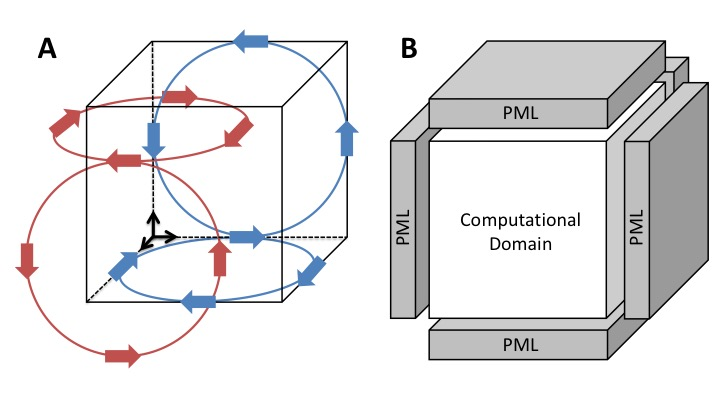
\includegraphics[width=\textwidth]{./Figures/Methods_Figure.jpg}
    \caption{a) Yee Grid b) Perfectly matched layer boundary condition}
    \label{fig:YeePML}
\end{figure}

\subsection{Finite Difference Time Domain}

A method called Finite Difference Time Domain uses finite differences (Appendix A) to solve the partial differential equations presented in the last section. Finite differencing is fairly common practice in numerical methods, but solving Maxwell's Equations in this way is unique because there are two interdependent fields to be updated in time. The way in which we construct the numerics forces the electromagnetic field to propagate as a wave, a physically realistic
representation. 

\subsubsection{Yee Grid}

To start, we want to lay out a grid on which the numerical problem will be solved. We will start in three dimensions, but eventually simplify the problem into lower dimensionality.

The most common technique here is to use what is called a Yee Grid (\cite{Yee1966}) which is staggered in both space and time. Staggering the grid in this way allows one to more easily calculate the curl. See Figure \ref{figYeePML}a, where the grid is shown. Here we can see that the circuits of the electic field naturally encircle vectors of the magnetic field, and the same is true in the opposite direction. This allows us to more easily update those vectors. 

The Yee grid is also staggered in time. There is only a half time step between the calculation of the magnetic field from the electric field. Likewise, half a time step takes place during the update of the electric field from that new magnetic field. This progressive stepping allows the electromagnetic wave to propagate in a physical manner.

Some attention must be given to numerical stability. The Courant-Friedrichs-Levy stability criterion (CFL) says that 

\begin{equation}
    \sqrt{(\Delta x)^2 + (\Delta y)^2 + (\Delta z)^2} > c \Delta t
\end{equation}

meaning that the time step is limited by the spatial grid. 

\begin{figure}
    \centering
    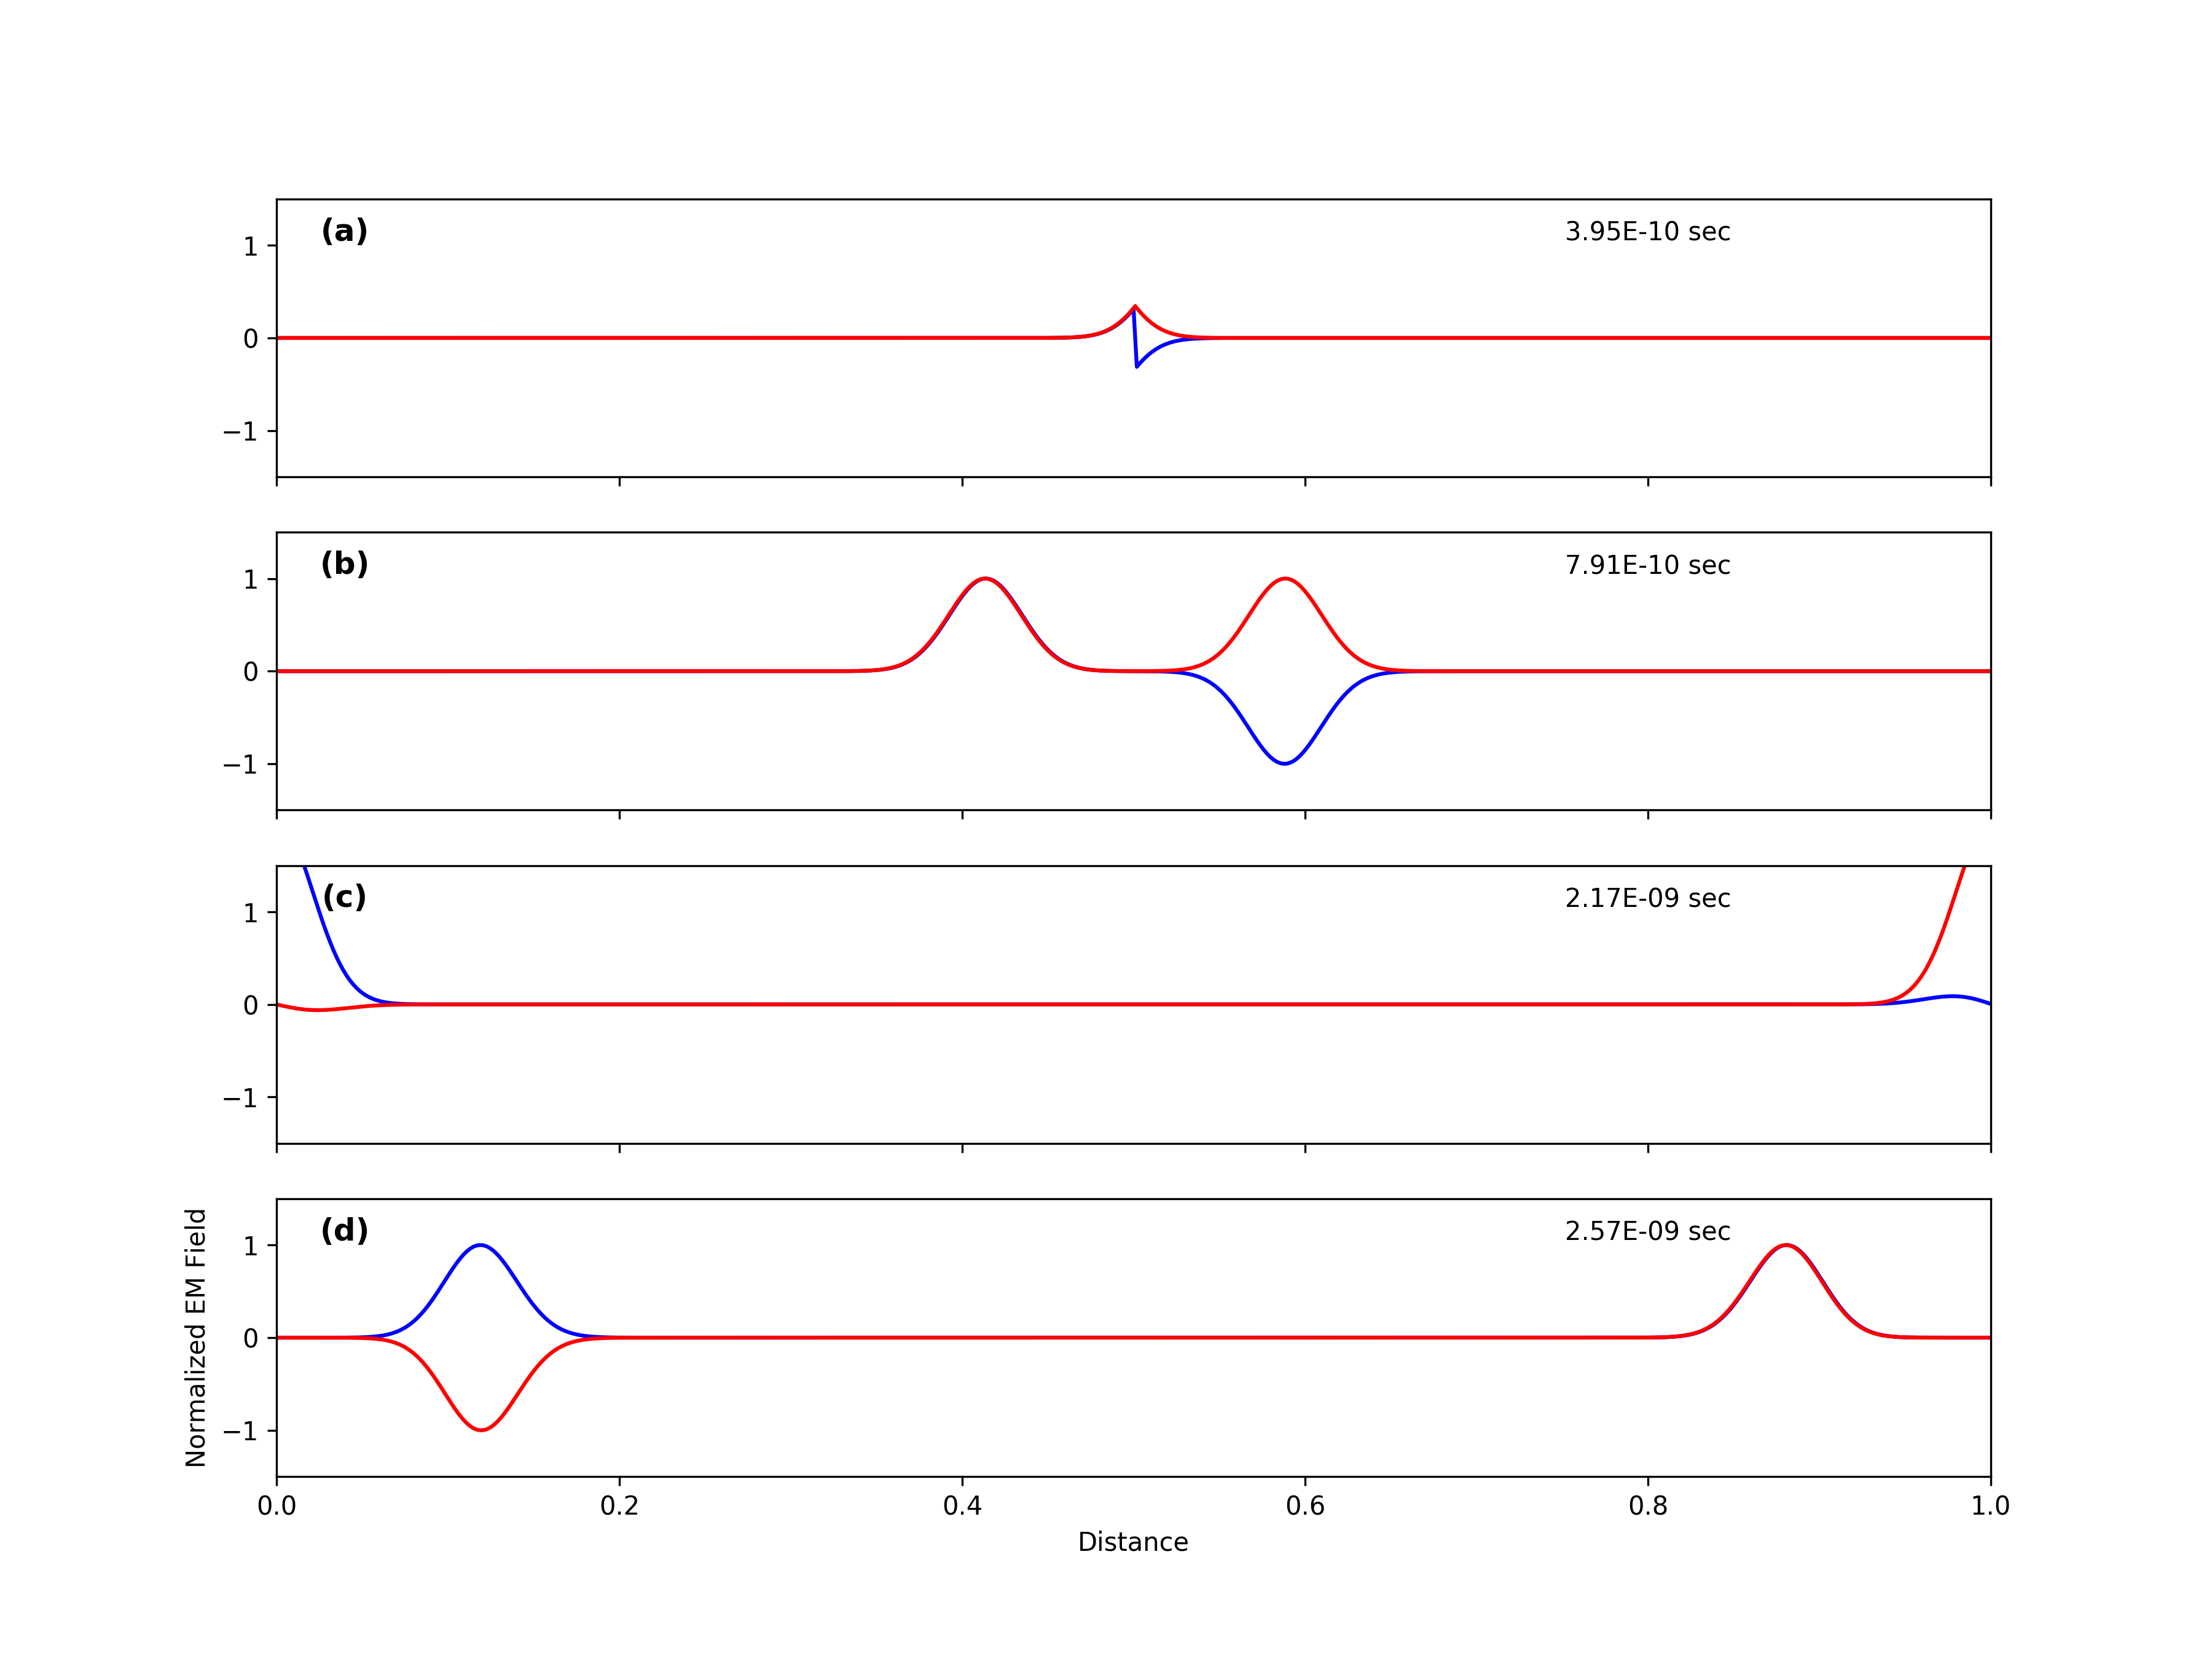
\includegraphics[width=\textwidth]{./Figures/DirichletBC.png}
    \caption{A sequence of plots for a one-dimensional finite difference time domain simulation with Dirichlet boundary conditions.}
    \label{fig:Dirichlet}
\end{figure}

\subsubsection{FDTD Modes}

Now we will break down the full three-dimensional problem description into some smaller more maneagable problems. First, we will assume that the off-diagonal components of the permeability and permittivity tensors are zero. Secondly, we will assume that there is no current in the material (i.e. $\textbf{J}=0$). 

The first model approximation that we want to address is in one dimension, and we will use z as our only direction. In this case, the equations break down into two usable groups [ref]. We will only show one here, the $E_y-H_x$ mode, but know that there is an analogous $E_x-H_y$ mode. The choice of one over another is unimportant in our case. For the $E_y-H_x$ mode, the equations reduce to,

\begin{equation}
    \frac{\partial E_y}{\partial z} = \mu_{xx} \frac{\partial H_x}{\partial t}
\end{equation}

\begin{equation}
    \frac{\partial H_x}{\partial z} = \epsilon_{yy} \frac{\partial E_y}{\partial t}
\end{equation}

Now we will use finite differences to write out update equations which can be implemented on a computer, 

\begin{equation}
    \frac{\left. E_y \right\vert_t^{k+1} - \left. E_y \right\vert_t^{k}}{\Delta z} = \mu_{xx}^{k} \frac{\left. H_x \right\vert_{t+\frac{\Delta t}{2}}^{k} - \left. H_x \right\vert_{t-\frac{\Delta t}{2}}^{k}}{\Delta t}
\end{equation}

\begin{equation}
    \frac{\left. H_x \right\vert_{t+\frac{\Delta t}{2}}^{k} - \left. H_x \right\vert_{t+\frac{\Delta t}{2}}^{k-1}}{\Delta z} = \epsilon_{yy}^{k} \frac{\left. E_y \right\vert_{t+\Delta t}^{k} - \left. E_y \right\vert_{t}^{k}}{\Delta t}
\end{equation}

Next, we will carry out a similar procedure for a two-dimensional model, in $E_z$ mode. In this case, we consider only the x and y directions. The magnetic field vectors will be solved in those same directions, but the electric field will be solved in the z-direction. 

\begin{equation}
    \frac{\partial E_z}{\partial y} = - \mu_{xx} \frac{\partial H_x}{\partial t}
\end{equation}

\begin{equation}
    \frac{\partial E_z}{\partial x} = \mu_{yy} \frac{\partial H_y}{\partial t}
\end{equation}

\begin{equation}
    \frac{\partial H_y}{\partial x} - \frac{\partial H_x}{\partial y} = \epsilon_{zz} \frac{\partial E_z}{\partial t}
\end{equation}

and again the numerical counterparts are

\begin{equation}
    \frac{\left. E_z \right\vert_{t}^{i,j+1} - \left. E_z \right\vert_{t}^{i,j}}{\Delta y} = - \mu_{yy}^{i,j} \frac{\left. H_y \right\vert_{t+\frac{\Delta t}{2}}^{i,j} - \left. H_y \right\vert_{t-\frac{\Delta t}{2}}^{i,j}}{\Delta t}
\end{equation}

\begin{equation}
    \frac{\left. E_z \right\vert_{t}^{i+1,j} - \left. E_z \right\vert_{t}^{i,j}}{\Delta x} = \mu_{xx}^{i,j} \frac{\left. H_x \right\vert_{t+\frac{\Delta t}{2}}^{i,j} - \left. H_x \right\vert_{t-\frac{\Delta t}{2}}^{i,j}}{\Delta t}
\end{equation}

\begin{equation}
    \frac{\left. H_y \right\vert_{t+\frac{\Delta t}{2}}^{i,j} - \left. H_y \right\vert_{t+\frac{\Delta t}{2}}^{i-1,j}}{\Delta x} - \frac{\left. H_x \right\vert_{t+\frac{\Delta t}{2}}^{i,j} - \left. H_x \right\vert_{t+\frac{\Delta t}{2}}^{i,j-1}}{\Delta y} = \epsilon_{zz}^{i,j} \frac{\left. E_z \right\vert_{t+1}^{i,j} - \left. E_z \right\vert_{t}^{i,j}}{\Delta t}
\end{equation}

\begin{figure}
    \centering
    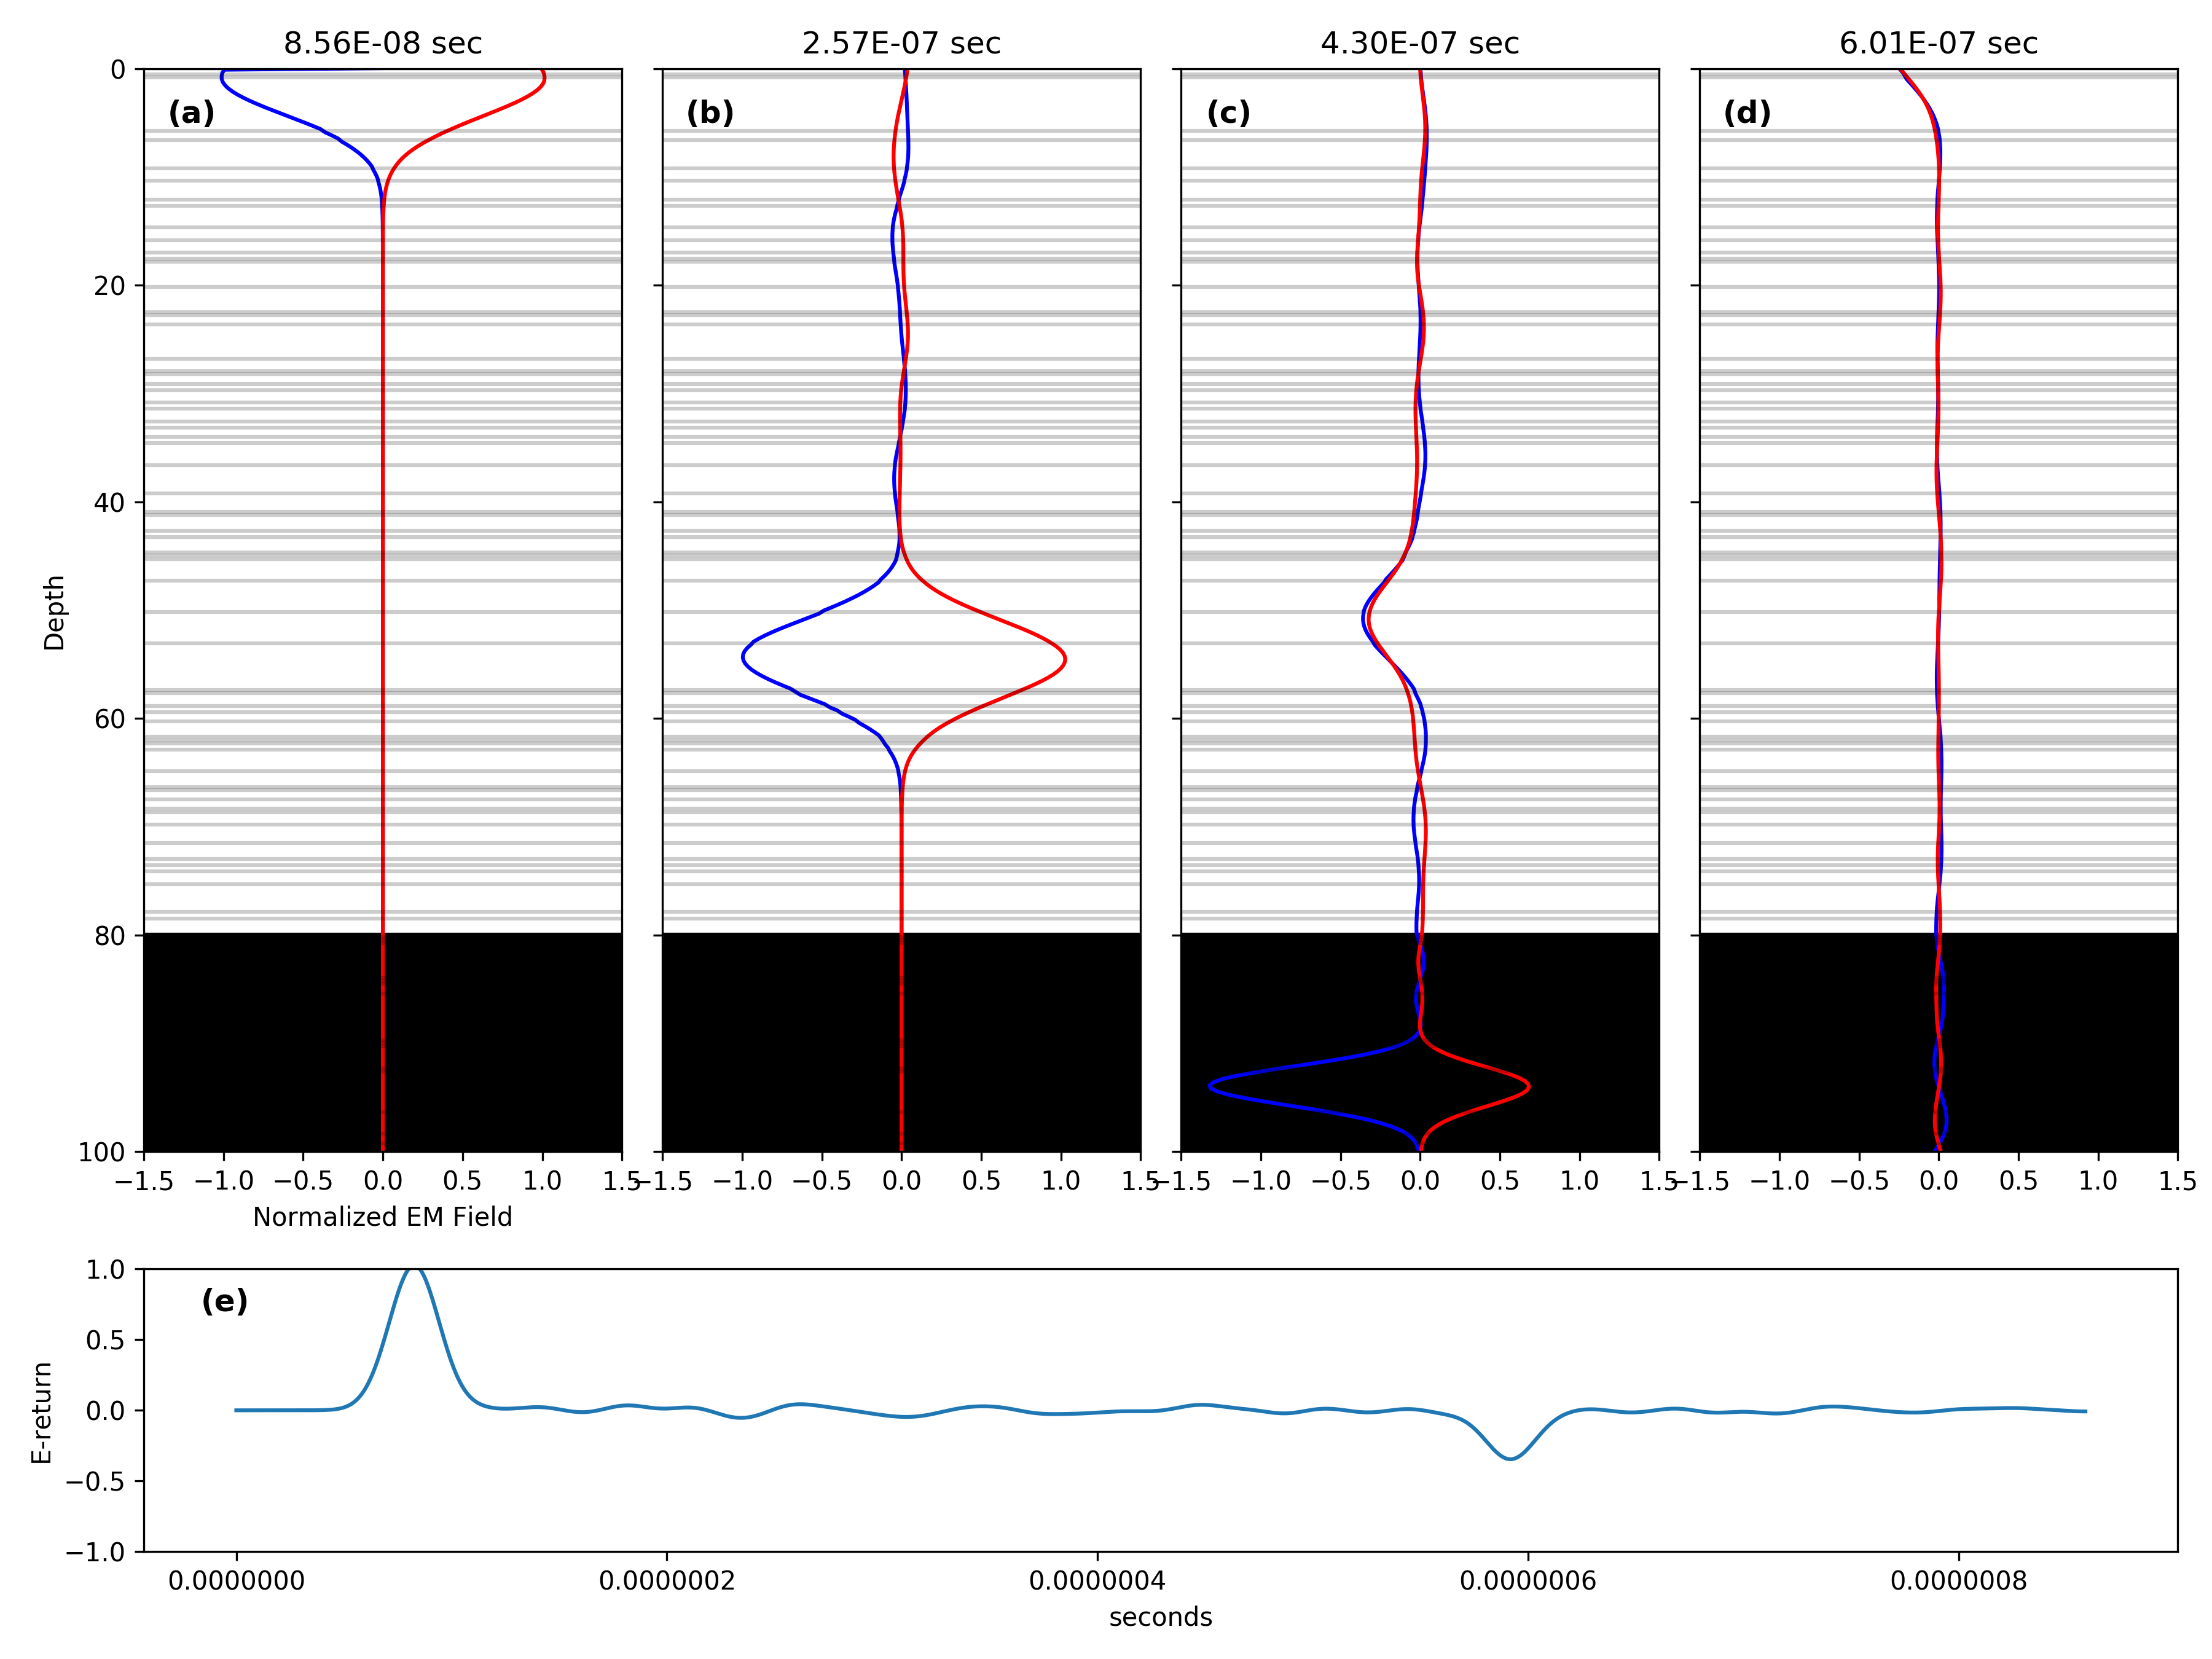
\includegraphics[width=\textwidth]{./Figures/IceSimulation.png}
    \caption{Simulation of EM wave propagation through ice.}
    \label{fig:Ice}
\end{figure}

\subsubsection{Boundary Conditions}

Now that we have defined our field equations and described the grid we must apply the boundary conditions. 

\begin{center}
    \colorbox[RGB]{239,240,241}{
    \begin{minipage}{.9\linewidth}
        \begin{algorithmic}[H]
            \For{x in range(x):}
            \State H+=1
            \EndFor
        \end{algorithmic}
    \end{minipage}}
\end{center}

PML in 2 or 3 dimensions

\section{Results}

The dirichlet boundary condition makes the wave bounce off the wall. The PML allows the wave to pass. 

Contrasts in permittivity create reflections. 

2d is pretty much the same as 1d but much more difficult to implement the PML condition. 

\begin{figure}
    \centering
    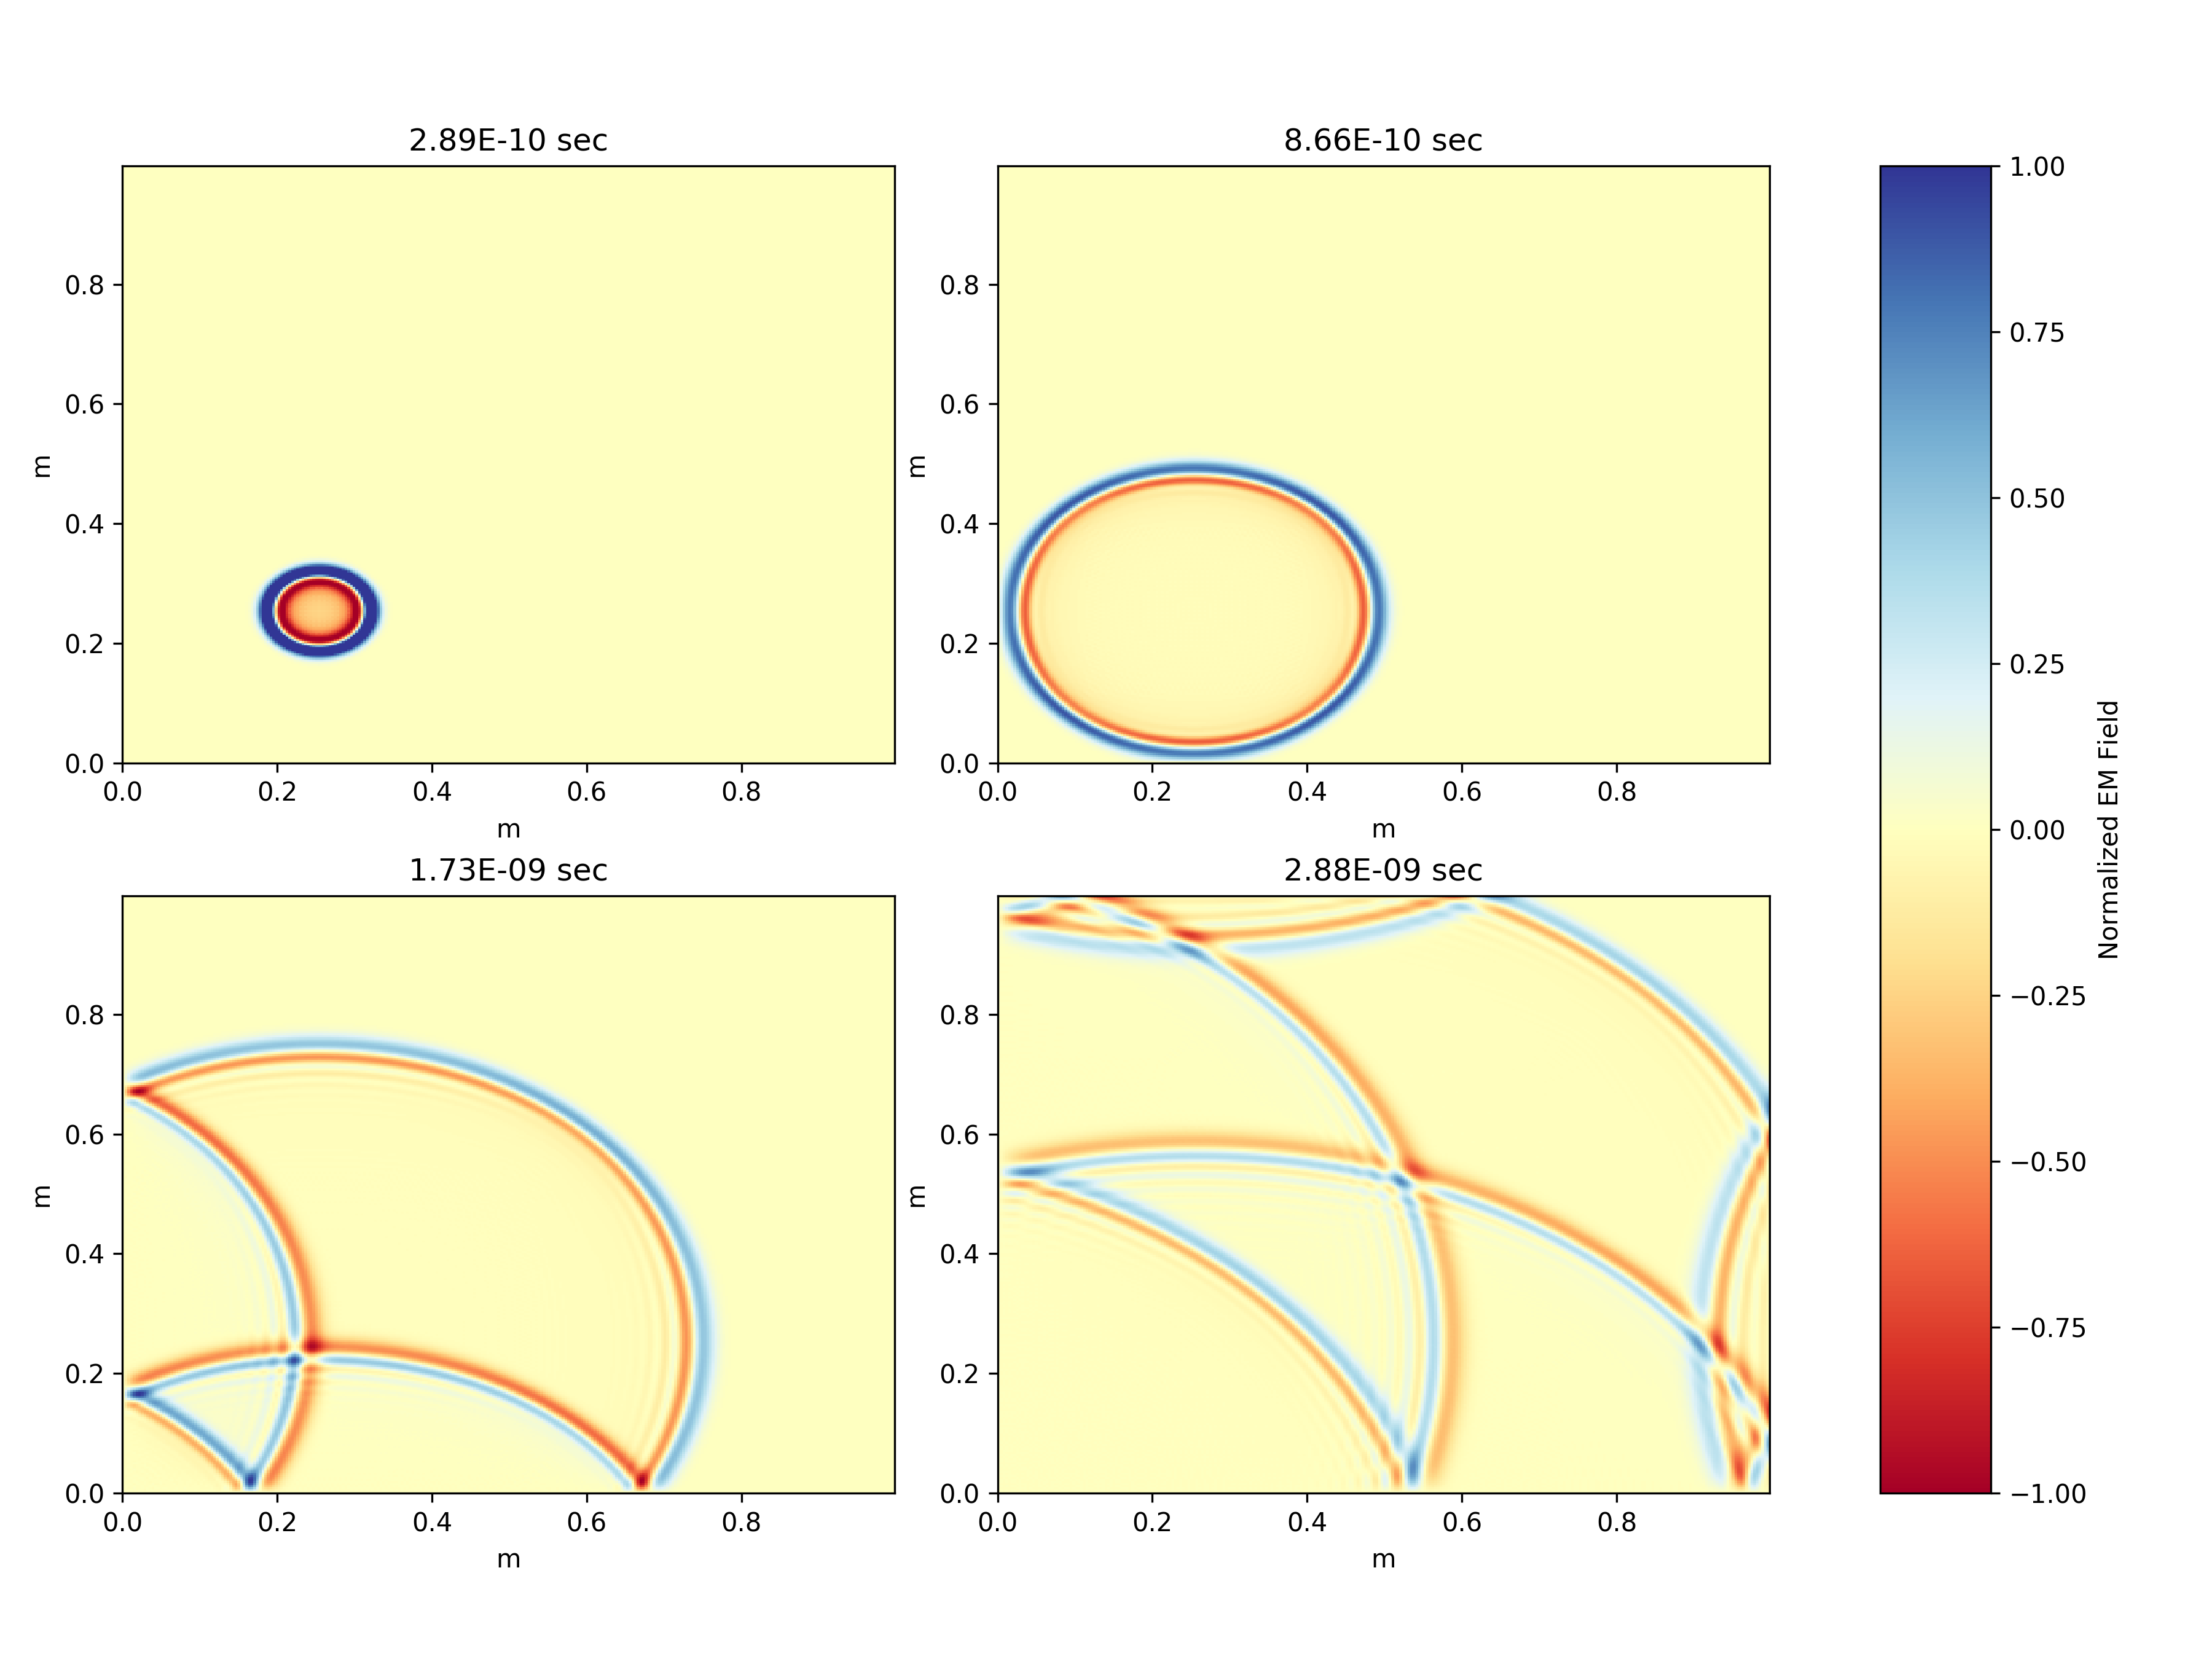
\includegraphics[width=\textwidth]{./Figures/2D_figure.png}
    \caption{Two-dimensional finite difference time domain.}
    \label{fig:2D}
\end{figure}

\section{Discussion}

RES methods are useful in many disciplines of geosciences. The let us uncover some information about that which we cannot see. The point of FDTD in my mind is to play around with ideas and see if they are viable. 

Layering, raymond bump.

Phase-based RES.

Attenuation and radiothermometry

\section{Conclusions}

\section{Appendix: Finite Difference Method}

One common way to solve partial differential equations numerically is with finite differences. This appendix is meant to give a brief overview of how this method works. Finite differencing uses the Taylor Series which approximates a function at some point, 

\begin{equation}
    f(x_i + \Delta x_i) = f(x_i) + \Delta x_i \left. \frac{\partial f}{\partial x} \right\vert_{x_i} + \frac{\Delta x_i^2}{2!} \left. \frac{\partial^2 f}{\partial x^2} \right\vert_{x_i} + \dots
\end{equation}

From the Taylor Series above, we can solve for any order derivative by simply moving terms around. 

\begin{equation}
    \left. \frac{\partial f}{\partial x} \right\vert_{x_i} = \frac{f(x_i + \Delta x_i) - f(x_i)}{\Delta x_i} + O(\Delta x_i)
\end{equation}

\section*{Data Availability}

Model scripts are available for download as a git repository at \url{https://github.com/benhills/FDTD.git}.

\printbibliography

\end{document}
